\documentclass[a4paper,11pt]{article}

\usepackage[pdftex]{graphicx}
%\usepackage{babel}
\usepackage[utf8]{inputenc}
\usepackage[T1]{fontenc}
%\usepackage[T1,mtbold,lucidacal,mtplusscr,subscriptcorrection]{mathtime}
\usepackage{times}
\usepackage{amsmath}
\usepackage{url}
\usepackage{enumerate}
\usepackage{parskip}
\usepackage[colorlinks,urlcolor=black]{hyperref}
\usepackage{microtype}

% if not draft, smaller printable area makes the paper more readable
\topmargin -4mm
\oddsidemargin 0mm
\textheight 225mm
\textwidth 150mm

%\parskip=\baselineskip

\DeclareMathOperator{\E}{E}
\DeclareMathOperator{\Var}{Var}
\DeclareMathOperator{\var}{var}
\DeclareMathOperator{\Sd}{Sd}
\DeclareMathOperator{\sd}{sd}
\DeclareMathOperator{\Bin}{Bin}
\DeclareMathOperator{\Beta}{Beta}
\DeclareMathOperator{\Poisson}{Poisson}
\DeclareMathOperator{\betacdf}{betacdf}
\DeclareMathOperator{\Invchi2}{Inv-\chi^2}
\DeclareMathOperator{\logit}{logit}
\DeclareMathOperator{\N}{N}
\DeclareMathOperator{\U}{U}
\DeclareMathOperator{\tr}{tr}
\DeclareMathOperator{\trace}{trace}

% Parenthesis \left  \right -fix
\renewcommand*{\l}{\mathopen{}\mathclose\bgroup\left}
\renewcommand*{\r}{\aftergroup\egroup\right}


% Horizontal line
\newcommand{\HRule}{\rule{\linewidth}{0.5mm}}

% \pagestyle{empty}


% Stan source code block
\usepackage{listings}


\begin{document}
% \thispagestyle{empty}

\section*{Bayesian data analysis -- exercise 7}

%This assignment is related to Chapter 11

The maximum amount of points from this assignment is 6. In addition to the correctness of the answers, the overall quality and clearness of the report is evaluated.

Report all results to a single, {\bf anonymous} *.pdf -file and return it to \href{peergrade.io}{peergrade.io}. Include also source code to the report (either as an attachment or as a part of the answer). By anonymity it is meant that the report should not contain your name or student number.

\HRule

\vspace{1cm}


\subsection*{1. Linear model: drowning data with Stan (3p)}

The provided {\tt drowning.txt} file contains the number of people drown per year in Finland 1980--2016.
%We build a linear model using time as the predictor to explain the changes in the number of people drown. with Gaussian noise
We are going to fit a linear model with Gaussian noise to these data using time as the predictor and number of drownings as the target variable (see related linear model example for the Kilpisjärvi-temperature data in the example Stan codes).
We have two objective questions:
\begin{itemize}
	\item [i)] What can you say about the trend in the number of people drown per year? We would plot the histogram of the slope of the linear model.
	\item [ii)] What does the model predict for year 2019? We would plot the histogram of the posterior predictive distribution for number of people drown at $\tilde x=2019$.
\end{itemize}

The provided Stan code in Listing~\ref{listing1} is almost correct for the given problem. However, there are two crucial mistakes. Find these two mistakes and fix them. Report the original mistakes and your fixes clearly in your report.

The provided broken code does not define any prior for the parameters. In Stan, this corresponds to using a uniform prior. We would like to apply a weakly-informative prior $\operatorname{N}(0, \tau^2)$ for the slope parameter {\tt beta}. It is very unlikely that the mean number of drownings changes more than 50 \% in one year. The approximate historical mean yearly number of drownings is 138. Hence, set $\tau$ so that the prior probability for {\tt beta} being less than $-69$ or greater than $69$ is $0.01$. Report suitable approximate numerical value for $\tau$ and clearly indicate how one would implement this in the Stan code.

Example resulting plots for the problem, with the fixes and the desired prior applied, are shown in Figure~\ref{fig1}. If you want, you can use these plots as a reference for testing if your modified Stan code produces similar results. However, running the inference and comparing the plots is not required. In the report, in addition to the full resulting Stan model code, the following things needs to be clearly presented and discussed in separate sections:
\begin{itemize}
\item the fixes in the code,
\item suitable approximate numerical value for $\tau$,
\item details how to implement the desired prior in the code.
\end{itemize}

\begin{lstlisting}[
	float,
	caption=Broken Stan code for question 1,
	label=listing1,
	basicstyle=\footnotesize\ttfamily,
	numbers=left,
	xleftmargin=2.7em,
	frame=single,
	framexleftmargin=2.2em
]
data {
    int<lower=0> N;  // number of data points
    vector[N] x;     // observation year
    vector[N] y;     // observation number of drowned
    real xpred;      // prediction year
}
parameters {
    real alpha;
    real beta;
    real sigma;
}
transformed parameters {
    vector[N] mu;
    mu = alpha + beta*x;
}
model {
    y ~ normal(mu, sigma);
}
generated quantities {
    real ypred;
    ypred = normal_rng(mu, sigma);
}
\end{lstlisting}

\begin{figure}
\centering
   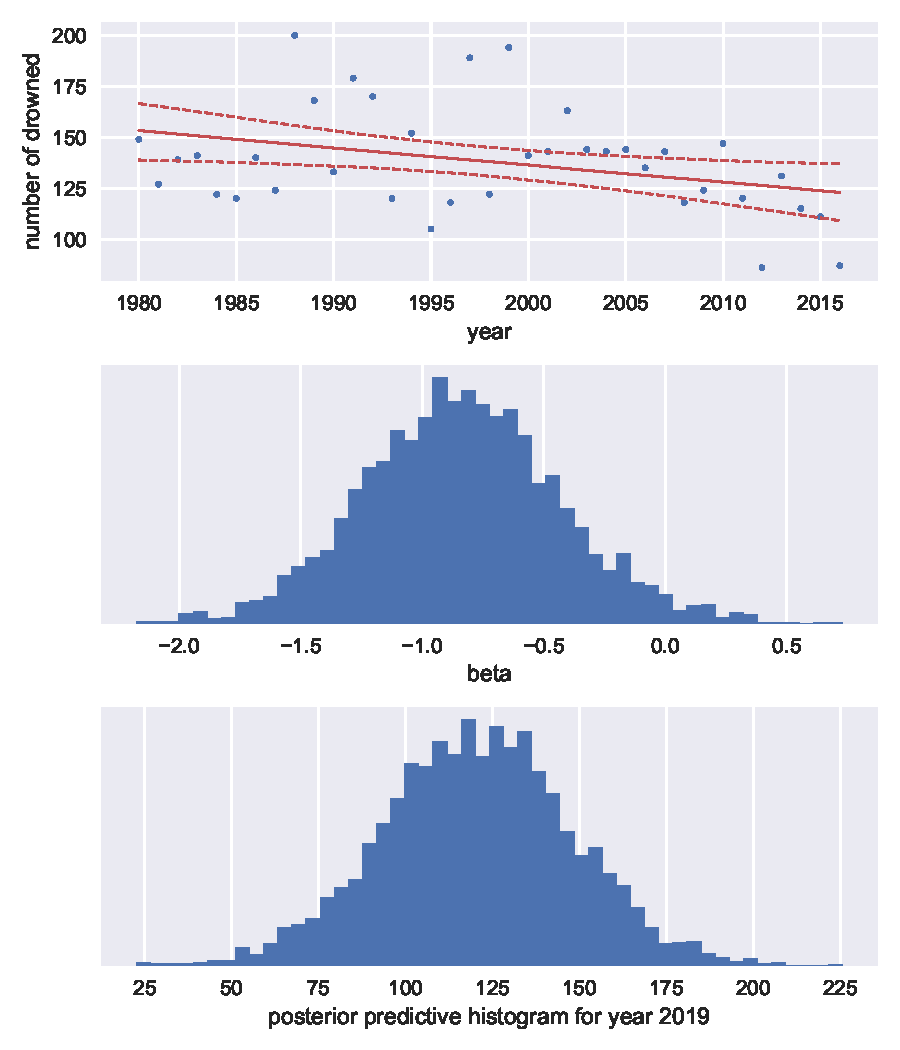
\includegraphics[width=0.66\textwidth]{ex7_fig1.pdf}
\caption{Example plots for the results obtained for problem in the question 1.}\label{fig1}
\end{figure}


\subsection*{2. Hierarchical model: factory data with Stan (3p)}

The provided {\tt factory.txt} file contains quality control measurements from 6 machines in a factory (units of the measurements are irrelevant here). In the data file, each column contains the measurements for a single machine. Quality control measurements are expensive and time-consuming, so only 5 measurements were done for each machine. In addition to the existing machines, we are interested in the quality of another machine (the seventh machine).

Implement a separate, pooled and hierarchical Gaussian model described in Section 11.6 using Stan. In the pooled model, all the measurements are combined together and no distinction is made between the machines. In the separate model, each machine has its own model. Similarly as in the model description in the book, use the same measurement standard deviation $\sigma$ for all the groups in the hierarchical model. In the separate model however, use separate measurement standard deviation $\sigma_j$ for each group $j$. Use Stan's default uniform prior for all the parameters.

Using each of the three models -- separate, pooled, and hierarchical -- report (comment and, if applicable, plot histogram):
\begin{itemize}
	\item [i)] the posterior distribution of the mean of the quality measurements of the sixth machine
	\item [ii)] the predictive distribution for another quality measurement of the sixth machine
	\item [iii)] the posterior distribution of the mean of the quality measurements of the seventh machine.
\end{itemize}

Hint:
See the example Stan-codes for the comparison of $k$ groups with and without the hierarchical structure. What you need to do is change the dataset, implement the prediction for the future measurement of the sixth machine, and figure out the distribution for the mean of the quality measurements for the seventh machine in the hierarchical model.

\end{document}

%%% Local Variables:
%%% mode: latex
%%% TeX-master: t
%%% End:
